\documentclass[10pt,a4paper]{article}
\usepackage[T1]{fontenc}
\usepackage{lmodern,microtype,graphicx,booktabs,tabularx,xcolor}
\usepackage[margin=20mm,top=17mm,bottom=18mm,footskip=9mm]{geometry}
\usepackage[colorlinks=true,urlcolor=teal!60!black]{hyperref}
\usepackage{fancyhdr}
\definecolor{ink}{HTML}{162E38}
\definecolor{accent}{HTML}{076B71}
\definecolor{muted}{HTML}{48616B}
\setlength{\parindent}{0pt}
\setlength{\parskip}{5pt}
\raggedbottom
\pagestyle{fancy}\fancyhf{}
\renewcommand{\headrulewidth}{0pt}
\lfoot{\footnotesize\sffamily\color{muted}Public observations\enspace/\enspace20 November 2026}
\rfoot{\footnotesize\sffamily\color{muted}\thepage}
\newcommand{\kicker}[1]{{\sffamily\small\bfseries\color{accent}#1}\par\vspace{5pt}}
\newcommand{\headline}[1]{{\raggedright\sffamily\bfseries\color{ink}\fontsize{23}{26}\selectfont #1\par}\vspace{3pt}}
\newcommand{\sub}[1]{\par\vspace{3pt}{\sffamily\bfseries\large\color{ink}#1}\par}
\newcommand{\captiontext}[1]{{\small\color{muted}#1}\par}
\begin{document}
\color{ink}
\kicker{GLACIOLOGY \hfill WESTERN GREENLAND ICE SHEET}
\headline{A 5.38 square kilometre loss of open water in a Greenland lake basin}
Within a fixed 4.0 by 3.2\,km window at $67.12718^\circ$\,N, $48.53845^\circ$\,W, open water expanded from 1.68 to 5.82\,km$^2$ between 16 and 20 July 2026. On 23 July, 0.44\,km$^2$ remained in that window. A second optical satellite and a radar satellite independently tracked the change.

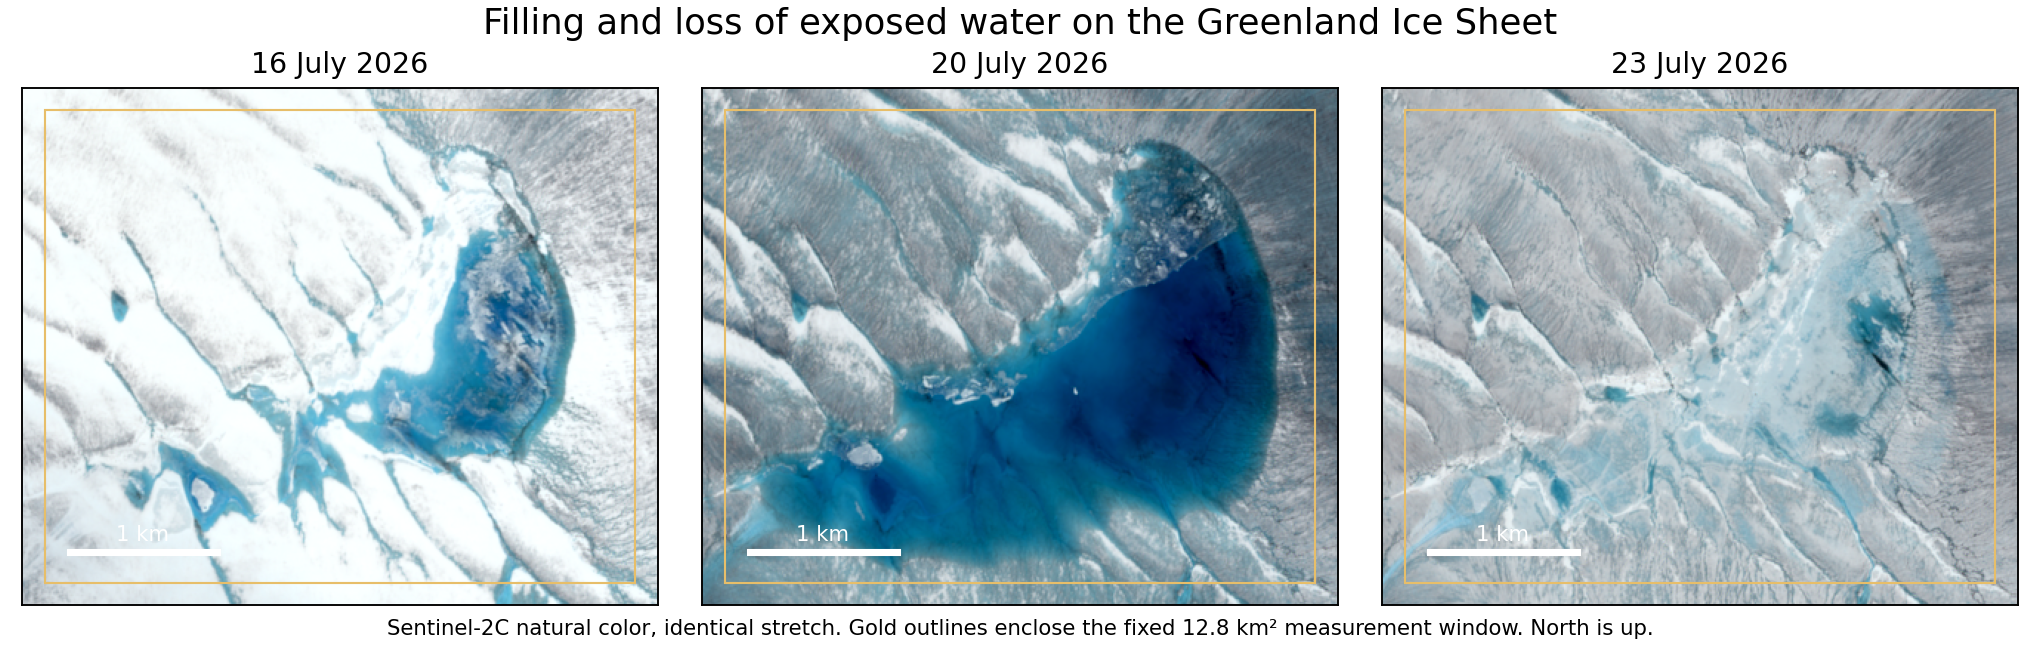
\includegraphics[width=\linewidth]{lake-sequence.png}

\sub{What the satellites establish}
\begin{tabularx}{\linewidth}{@{}l l X@{}}\toprule
Date (UTC) & Instrument & Observation in the basin\\\midrule
20 July, 14:54 & Sentinel-2C & 5.819\,km$^2$ of water in a cloud-free image.\\
21 July, 14:55 & Landsat 9 & At least 4.465\,km$^2$ of water, with 72\% of the window clear.\\
22 July, 09:36 & Sentinel-1C & 68.7\% of the peak footprint had low radar backscatter relative to nearby ice.\\
23 July, 14:43 & Landsat 9 & 0.413\,km$^2$ of water in a clear image.\\
23 July, 15:04 & Sentinel-2C & 0.442\,km$^2$, down 92.4\% in 72 hours 10 minutes.\\\bottomrule
\end{tabularx}

The last widespread radar signature and first clear view of the depleted basin were 29 hours 7 minutes apart. This brackets the transition between those two observed states. The start, duration and drainage route remain unresolved.

\sub{How sensitive is the result?}
Water area counts cloud-masked pixels inside the gold rectangle. Connected pools and channels extend beyond it. Varying the blue--red normalized-difference threshold from 0.20 to 0.30 changes the estimated area loss from 88.0\% to 94.5\%. One pool 3.5\,km southeast retained a water signature across 92\% of its sampled interior on 23 July. At weather station KAN\_M, 15.38\,km away, all 29 hourly air temperatures inside the radar-to-optical interval were positive ($+0.26$ to $+2.22^\circ$C). The station provides regional context. The observations do not measure discharged volume.

\sub{Which part may be new?}
Published polygons overlap this basin in 2018 and 2019. The finding is the timing and extent of its July 2026 loss. No matching event report surfaced in the inventories and literature examined by 20 November 2026. Unpublished work and later catalog updates remain possible.

\captiontext{Data: Copernicus Sentinel-1/2, USGS/NASA Landsat 9, and GEUS PROMICE/GC-Net. \href{https://earth-search.aws.element84.com/v1/collections/sentinel-2-l2a/items/S2C_22WFV_20260720_0_L2A}{20 July Sentinel-2 scene}\enspace$\cdot$\enspace\href{https://earth-search.aws.element84.com/v1/collections/sentinel-2-l2a/items/S2C_22WFV_20260723_0_L2A}{23 July scene}\enspace$\cdot$\enspace\href{https://zenodo.org/records/16577959}{Historical lake polygons (Glen et al.)}\enspace$\cdot$\enspace\href{https://thredds.geus.dk/thredds/dodsC/aws/l3sites/netcdf/hour/KAN_M_hour.nc.html}{KAN\_M observations}.}

\end{document}
